\section{Typed realizability}
\label{sec:typed-realizability}

RZ is based on \emph{typed realizability} by John
Longley~\cite{Longley99}.   This variant of realizability corresponds most
directly to programmers' intuition about implementations.

We approach typed realizability and its relationship to
real-world programming by way of example. Suppose we are asked to
design a data structure for the set $\mathcal{G}$ of all finite
simple%
\iflong
\footnote{At most one arrow between any two vertices.}
\fi % \iflong
\ directed graphs with vertices labeled by distinct integers. 
%
\iflong
An exemplar
directed graph~$G$ is shown in Figure~\ref{fig:digraph}.
%
\begin{figure}
  \centering
  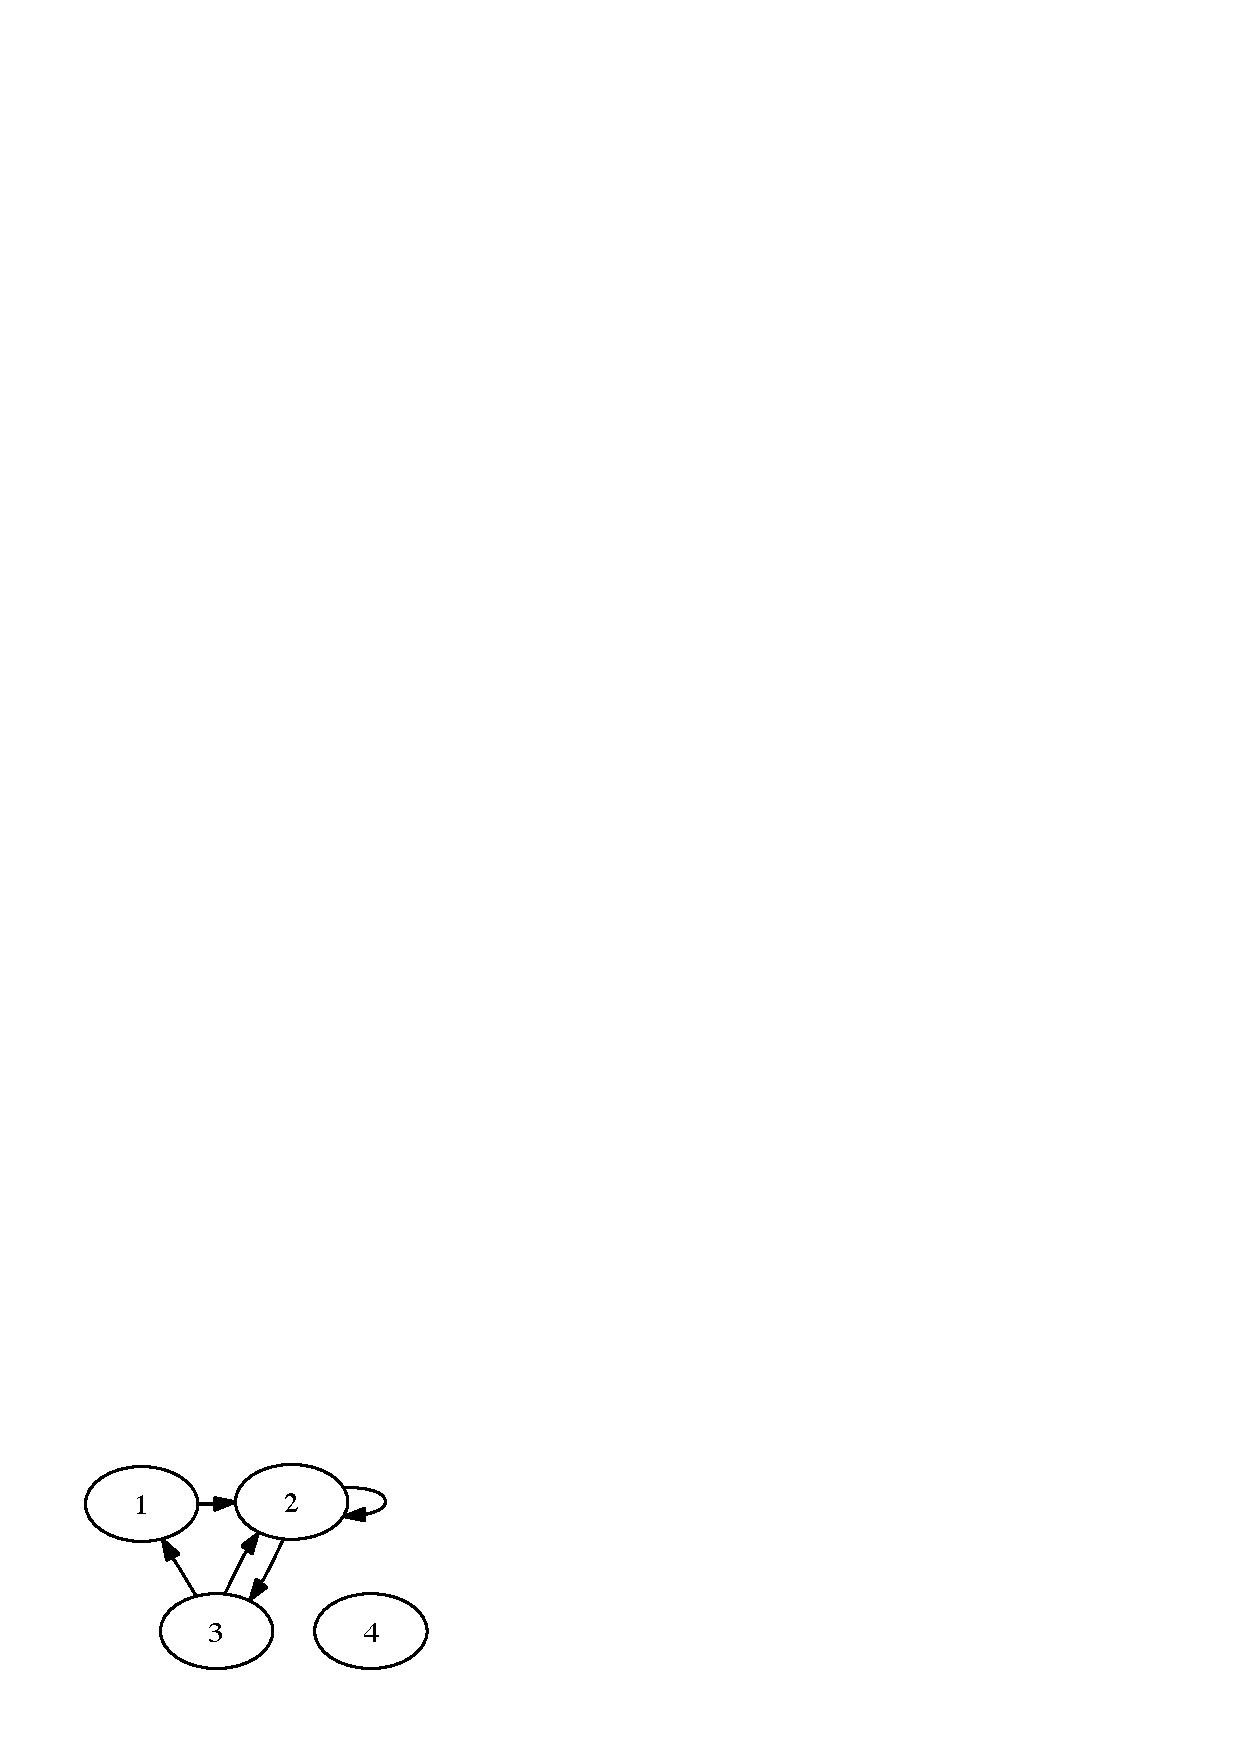
\includegraphics[width=0.3\textwidth]{digraph}
  \caption{A finite directed graph $G$}
  \label{fig:digraph}
\end{figure}
\fi % \iflong
%
A common representation is a pair of lists $(\ell_V, \ell_A)$, where
$\ell_V$ is the list of vertex labels and $\ell_A$ is the \emph{adjacency list} 
representing the arrows by pairing the labels of each source and target.
\iflong
In our example,
$\ell_V = [1; 2;
3; 4]$ and $\ell_A = [(1,2); (2,2); (2,3); (3,2); (3;1)]$.
\fi % \iflong
%
Thus we define the datatype of graphs as\footnote{We use OCaml
  notation in which $\clist{t}$ classifies finite lists of elements of
  type~$t$, and $t_1 * t_2$ classifies pairs containing a value of
  type $t_1$ and and value of type $t_2$.}
%
\begin{equation*}
  \ctype \mathtt{graph} = \clist{\cint} \ \ * \ \ \clist{(\cint * \cint)}
\end{equation*}
%
However, this is not a complete description of the representation, as
there would be representation invariants and conditions not expressed by the type, e.g.,
%
\iflong
\begin{enumerate}
\item The order in which vertices and arrows are listed is not
  important%
; for example, $[1;2;3;4]$ and $[4;1;2;3]$ represent the same vertices.
\item Each vertex and arrow must be listed exactly once.
\item The source and target of each arrow must appear in the list of vertices.
\end{enumerate}
\else % \iflong
the order in which vertices and arrows are listed is not
important, each vertex and arrow must be listed exactly once, and
the source and target of each arrow must appear in the list of vertices.
\fi %\iflong

%
Thus, to implement the mathematical set~$\mathcal{G}$, we must not
only decide on the underlying datatype $\mathtt{graph}$, but also
determine what values of that type represent which elements
of~$\mathcal{G}$. As we shall see next, this can be expressed either
using a \emph{realizability relation} or a \emph{partial equivalence
  relation (per)}.


\subsection{Modest sets and pers}
\label{sec:modest-sets-pers}

\iflong
We now define typed realizability as it
applies to OCaml. Other general-purpose programming languages could be
used instead, as long as they provide the usual ground types, product
and function types.\footnote{It is also convenient to work with a
language that supports sum types, as this allows a more natural
representation of disjoint unions.}
\else
We now define typed realizability as it
applies to OCaml. Other general-purpose programming languages could be
used instead.
\fi % \iflong

Let $\Type$ be the collection of all (non-parametric) OCaml types. To
each type $t \in \Type$ we assign the set $\values{t}$ of values of
type~$t$ that behave \emph{functionally} in the sense of
Longley~\cite{longley99when}. Such values are represented by
terminating expressions that do not throw exceptions or return
different results on different invocations. They may \emph{use}
exceptions, store, and other computational effects, provided they
appear functional from the outside; a useful example using
computational effects is presented in
Section~\ref{sec:we-show-modulus-of-continuity-example}. A functional
value of function type may diverge as soon as it is applied. The
collection $\Type$ with the assignment of functional values
$\values{t}$ to each $t \in \Type$ forms a \emph{typed partial
  combinatory algebra (TPCA)}%
\iflong
, which provides a theoretical basis for
the definition of a realizability model that suits our needs%
\fi%\iflong
.

Going back to our example, we see that an implementation of directed
graphs $\mathcal{G}$ specifies a datatype $\typeOf{\mathcal{G}} =
\mathtt{graph}$ together with a \emph{realizability relation}
$\rz_{\mathcal{G}}$ between $\mathcal{G}$ and
$\values{\mathtt{graph}}$. The meaning of $(\ell_V, \ell_A)
\rz_\mathcal{G} G$ is ``OCaml value $(\ell_V, \ell_A)$
represents/realizes/implements graph $G$''.
%
\iflong
%
There are two natural
conditions that $\rz_\mathcal{G}$ ought to satisfy: (1) for every $G
\in \mathcal{G}$ there should be at least one realizer $(\ell_V,
\ell_A)$ representing it, and (2) if $(\ell_V, \ell_A)$ represents
both $G$ and $G'$ then $G = G'$.\footnote{The latter condition is
  called \emph{modesty} and is not strictly necessary for the
  development of the theory, though programmers would naturally expect
  it to hold.} If $(\ell_V, \ell_A)$ and $(\ell'_V, \ell'_A)$
represent the same graph (e.g., because $\ell_V$ is a permutation of
$\ell'_V$, and similarly for $\ell_A$ and $\ell'_A$) we say that they
are \emph{equivalent} and write $(\ell_V, \ell_A) \per_\mathcal{G}
(\ell'_V, \ell'_A)$. The relation $\per_\mathcal{G}$ is a
\emph{partial} equivalence relation (symmetric and transitive, but not
reflexive) because not every $(\ell_V, \ell_A) \in
\values{\mathtt{graph}}$ represents a graph.

\smallskip

A general definition is in order. A \emph{modest set} is 
%
\else % iflong
%
Generalizing from this, we define a \emph{modest set} to be
%
\fi
%
a triple $A = (\setOf{A}, \typeOf{A}, {\rz_A})$ where $\setOf{A}$ is
the \emph{underlying set}, $\typeOf{A} \in \Type$ is the
\emph{underlying type}, and $\rz_A$ is a \emph{realizability relation}
between $\values{\typeOf{A}}$ and $\setOf{A}$, satisfying
%
\iflong
% 
\begin{enumerate}
\item \emph{totality:} for every $x \in \setOf{A}$ there is $v \in
  \values{\typeOf{A}}$ such that $v \rz_A x$, and
\item \emph{modesty:} if $u \rz_A x$ and $u \rz_A y$ then $x = y$.
\end{enumerate}
%
\else % iflong
%
(1) \emph{totality:} for every $x \in \setOf{A}$ there is $v \in
\values{\typeOf{A}}$ such that $v \rz_A x$, and (2) \emph{modesty:} if
$u \rz_A x$ and $u \rz_A y$ then $x = y$.
%
\fi % iflong
%
The \emph{support} of $A$ is the set $\support{A} = \set{v \in
  \values{\typeOf{A}} \such \xsome{x}{\setOf{A}}{v \rz_A x}}$ of those
values that realize something. We define the relation $\per_A$ on
$\values{\typeOf{A}}$ by
%
\begin{equation*}
  u \per_A v
  \iff
  \some{x}{\setOf{A}}{u \rz_A x \land v \rz_A x} \;.
\end{equation*}
%
From totality and modesty of $\rz_A$ it follows that $\per_A$ is a per,
i.e., symmetric and transitive. Observe that $\support{A} = \set{v \in
  \values{\typeOf{A}} \such v \per_A v}$, whence $\per_A$
restricted to $\support{A}$ is an equivalence relation. In fact, we
may recover a modest set up to isomorphism from $\typeOf{A}$ and
$\per_A$ by taking $\setOf{A}$ to be the set of equivalence classes of
$\per_A$, and $v \rz_A x$ to mean $v \in x$.

The two views of implementations, as modest sets $(\setOf{A},
\typeOf{A}, {\rz_A})$, and as pers $(\typeOf{A}, {\per_A})$, are
equivalent.\footnote{And there is a third view, as a partial surjection
  $\delta_A : {\subseteq}\values{\typeOf{A}} \epito \setOf{A}$, with
  $\delta_A(v) = x$ when $v \rz_A x$. This is how realizability is
  presented in Type Two Effectivity~\cite{Wei00}.} 
%
We concentrate on the view of modest sets as pers. They are more
convenient to use in RZ because they refer only to types and values,
as opposed to arbitrary sets.
%
Nevertheless, it is useful to understand
how modest sets and pers arise from natural programming practice.

\iflong
%
Modest sets form a category whose objects are modest sets and
morphisms are the realized functions. A \emph{realized function} $f :
A \to B$ is a function $f : \setOf{A} \to \setOf{B}$ for which there
exists $v \in \values{\typeOf{A} \to \typeOf{B}}$ such that, for all
$x \in \setOf{A}$ and $u \in \typeOf{A}$,
%
\begin{equation}
  \label{eq:rz-function-space}
  u \rz_A x \implies v\;u \rz_B f(x) \;.
\end{equation}
%
This condition is just a mathematical expression of the usual idea
that~$v$ is an implementation of~$f$ if it does to realizers
what~$f$ does to the elements they represent.
\fi

\iflong
The equivalent category of pers has as objects
\else
Pers form a category whose objects are
\fi
%
pairs $A = (\typeOf{A}, {\per_A})$ where $\typeOf{A} \in \Type$ and
$\per_A$ is a per on $\values{\typeOf{A}}$. A morphism $A \to B$ is
represented by a function $v\in \values{\typeOf{A} \to \typeOf{B}}$
such that, for all $u, u' \in \support{A}$,
%
\iflong
\begin{equation}
  \label{eq:per-exponential}
  u \per_A u' \implies v\;u \per_B v\;u' \;.
\end{equation}
%
Values $v$ and $v'$ that both satisfy~\eqref{eq:per-exponential}
\else % \iflong
$u \per_A u' \implies v\;u \per_B v\;u'$.  Two such functions $v$ and $v'$
\fi
represent the same morphism if, for all $u, u' \in \support{A}$,
$u \per_A u'$ implies $v\;u \per_B v'\;u'$.

\iflong
%
The category of pers has a very rich structure. For example, we may
form a cartesian product $A \times B$ of pers $A$ and $B$ by
%
\begin{align*}
  \typeOf{A \times B} &= \typeOf{A} * \typeOf{B},\\
  (u_1, v_1) \per_{A \times B} (u_2, v_2) &\iff
  u_1 \per_A u_2 \land v_1 \per_B v_2.
\end{align*}
%
The projections $\pi_1 : A \times B \to A$ and $\pi_2 : A \times B \to
B$ are realized by $\mathtt{fst}$ and $\mathtt{snd}$, respectively.

The morphisms between pers~$A$ and~$B$ again form a per
$B^A$, also written as $A \to B$, called the \emph{exponential} of~$A$
and~$B$, with
%
\begin{align*}
  \typeOf{B^A} &= \typeOf{A} \to \typeOf{B},\\
  \support{B^A} &=
  \set{v \in \values{\typeOf{A} \to \typeOf{B}} \such 
    \all{u,u'}{\values{\typeOf{A}}}{u \per_A u' \implies v\,u \per_B v\,u'}}
  \\
  u \per_{B^A} v &\iff u, v \in \support{A} \land
  \xall{w}{\support{A}}{u\;w \per_B v\;w}.
\end{align*}
%
The evaluation map $e : B^A \times A \to B$ is realized by OCaml
application, $\cfun{(u,v)}{u\;v}$. If a function $f : C \times A \to
B$ is realized by $v$, then its transpose $\tilde{f} : C \to B^A$,
$\tilde{f}(z)(x) = f(z,x)$, is realized by $\cfun{z\;x}{v \; (z,x)}$.
This shows that the category of pers is cartesian closed. In
Section~\ref{sec:transl-sets-terms} we review other canonical
constructions on modest sets.

\bigskip
\else % \iflong
%
The category of pers has a very rich structure, namely that of a
regular locally cartesian closed category~\cite{Bauer:00}. This
suffices for the interpretation of first-order logic and (extensional)
dependent types~\cite{JacobsB:cltt}.
%
\fi % \iflong

\iflong
%
As an example we consider the cyclic group on seven elements $(\ZZ_7,
0, {-}, {+})$. To implement the group, we must give a representation
of $\ZZ_7$ as a per~$Z = (\typeOf{Z}, {\per_Z})$, and
provide realizers for the neutral element~$0$, negation~$-$, and
addition~$+$. 

One possibility is to choose $\cint$ as the underlying type
$\typeOf{Z}$, and to let $\support{Z}$ be only the integers \texttt{0}
through \texttt{6}. Then negation and addition must work modulo
\texttt{7} (i.e., must return an integer in the range
\texttt{0}--\texttt{6} when given integers in this range). The neutral
element would be the integer constant \texttt{0}, and the equivalence
$\per_Z$ would be integer equality.

Alternatively, we could take $\cint$ as the underlying type
$\typeOf{Z}$, but let $\support{Z}$ include all integers. In this
case, negation and addition could be simply integer addition and
negation\footnote{Taking care to prevent integer
  overflow.}. Here the neutral element could be implemented as any
integer multiple of \texttt{7}, and the equivalence $\per_Z$ would be
equivalence-modulo-7.

Both of these pers happen to be \emph{decidable}, i.e., it can be
algorithmically decided whether two values represent the same element
of~$\ZZ_7$, by code for integer equality and code for integer
equivalence-modulo-7 respectively. \fi % \iflong

\iflong
%
Not all pers are decidable.
%
\else
%
Not all pers are \emph{decidable}, i.e., there may be no algorithm for deciding
when two values are equivalent.
%
\fi
%
Examples include implementations of semigroups with an undecidable
word problem~\cite{post47:_recur_unsol_probl_thue}%
\iflong, implementations of computable sets of integers (which might
be realized by membership functions of type $\cint\to\cbool$),\fi
\ and implementations of computable real numbers (which might be
realized by infinite Cauchy sequences).
%
\iflong
%
There is no presupposition that pers are computable
(implementable). We can require decidable equivalence by adding a
suitable axiom; see Section~\ref{sec:decidable-sets}. \fi

\subsection{Interpretation of logic}
\label{sec:interpretation-logic}

In the realizability interpretation of logic, each formula~$\phi$ is
assigned a set of \emph{realizers}, which can be thought of as
computations that witness the validity of~$\phi$. The situation is
somewhat similar, but not equivalent, to the propositions-as-types
translation of logic into type theory, where proofs of a
proposition correspond to terms of the corresponding type. More
precisely, to each formula~$\phi$ we assign an underlying type
$\typeOf{\phi}$ of realizers, but unlike the propositions-as-types
translation, not all terms of type $\typeOf{\phi}$ are necessarily
valid realizers for~$\phi$, and some terms that are realizers may not
correspond to any proofs, for example, if they denote partial
functions or use computational effects.

It is customary to write $t \rz \phi$ when $t \in
\values{\typeOf{\phi}}$ is a realizer for~$\phi$. The underlying types
and the realizability relation~$\rz$ are defined inductively on the
structure of~$\phi$; an outline is shown in Figure~\ref{fig:rz-logic}.
We say that a formula~$\phi$ is \emph{valid} if it has at least one
realizer.
%
\begin{figure*}[t]
	\footnotesize
  \textbf{Underlying types of realizers:}
\[
  \begin{array}{ll@{\qquad}ll}
    \typeOf{\itrue} &= \mathtt{unit} &
    \typeOf{\ifalse} &= \mathtt{unit} \\
    \typeOf{\iequal{x}{y}} &= \mathtt{unit} &
    \typeOf{\iand{\phi}{\psi}} &= \oprod{\typeOf{\phi}}{\typeOf{\psi}} \\
    \typeOf{\iimply{\phi}{\psi}} &= \oarrow{\typeOf{\phi}}{\typeOf{\psi}} &
    \typeOf{\ior{\phi}{\psi}} &=
    \osumtyx{\mathtt{or}_0}{\typeOf{\phi_0}}{\mathtt{or}_1}{\typeOf{\phi_1}} \\
    \typeOf{\iforall{x}{A}{\phi}} &= \oarrow{\typeOf{A}}{\typeOf{\phi}} &
    \typeOf{\iexists{x}{A}{\phi}} &= \oprod{\typeOf{A}}{\typeOf{\phi}}
  \end{array}
\]
  \textbf{Realizers:}
\[
  \begin{array}{ll}
    () \rz \itrue & \\
    () \rz \iequal{x}{y}
    &\quad\text{iff}\quad 
    x = y
    \\
    (t_1,t_2) \rz \iand{\phi}{\psi}
    &\quad\text{iff}\quad
    \text{$t_1 \rz \phi$ and $t_2 \rz \psi$}
    \\
    t \rz \iimply{\phi}{\psi}
    &\quad\text{iff}\quad
    \text{for all $u \in \typeOf{\phi}$, if $u \rz \phi$ then $t\,u
      \rz \psi$}
    \\
    \oinj{\mathtt{or}_0}{t} \rz \ior{\phi}{\psi}
    &\quad\text{iff}\quad
    \text{$t \rz \phi$}
    \\
    \oinj{\mathtt{or}_1}{t} \rz \ior{\phi}{\psi}
    &\quad\text{iff}\quad
    \text{$t \rz \psi$}
    \\
    t \rz \iforall{x}{A}{\phi(x)}
    &\quad\text{iff}\quad
    \text{for all $u \in \typeOf{A}$, if $u \rz_A x$ then $t\,u \rz \phi(x)$}
    \\
    (t_1, t_2) \rz \iexists{x}{A}{\phi(x)}
    &\quad\text{iff}\quad
    \text{$t_1 \rz_A x$ and $t_2 \rz \phi(x)$}
  \end{array}
\]
\vspace{-0.5cm}
  \caption{Realizability interpretation of logic (outline)}
  \label{fig:rz-logic}
\end{figure*}

In classical mathematics, a predicate on a set~$X$ may be viewed as a
subset of~$X$ or a (possibly non-computable) function $X \to \oProp$,
where $\oProp = \set{\ofalse, \otrue}$ is the set of truth values.
Accordingly, since in realizability propositions are witnessed by
realizers,
%
\iflong
a predicate~$\phi$ on a modest set~$A$ may be viewed as a
subset of $\setOf{A} \times \values{\typeOf{\phi}}$, or a (possibly
non-computable) function $\setOf{A} \times \values{\typeOf{\phi}} \to
\set{\ofalse, \otrue}$. In terms of pers, which is what RZ uses,
\fi
%
a predicate~$\phi$ on a per~$A = (\typeOf{A}, {\per_A})$ is a
(possibly non-computable) function $\phi : \values{\typeOf{A}} \times
\values{\typeOf{\phi}} \to \oProp$ that is
%
\iflong
\begin{itemize}
\item \emph{strict:} if $\phi(u,v)$ then $u \in \support{A}$, and
\item \emph{extensional:} if $\phi(u_1,v)$ and $u_1 \per_A u_2$ then
  $\phi(u_2,v)$.
\end{itemize}
\else % \iflong
\emph{strict} (if $\phi(u,v)$ then $u \in \support{A}$) 
and \emph{extensional} (if $\phi(u_1,v)$ and $u_1 \per_A u_2$ then
  $\phi(u_2,v)$).
\fi

\iflong
We illustrate how the realizability interpretation extracts the
computational content of a proposition. To make an interesting
example, suppose
\else % \iflong
Suppose
\fi % \iflong
we have implemented the real
numbers~$\RR$ as a per~$R = (\mathtt{real}, {\per_R})$, and
consider  
\iflong
the statement
that every cubic $x^3 + a x + b$ has a root,
%
\begin{equation}
  \label{eq:square-root}%
  \iforall{a}{R}{\iforall{b}{R}{\iexists{x}{R}{\iequal{x^3 + a x + b}{0}}}}.
\end{equation}
\else % \iflong
$\iforall{a}{R}{\iforall{b}{R}{\iexists{x}{R}{\iequal{x^3 + a x + b}{0}}}}$.
\fi % \iflong
%
By computing according to Figure~\ref{fig:rz-logic}, we see that
a realizer for this proposition is a value~$r$ of type
$\oarrow{\mathtt{real}}{\oarrow{\mathtt{real}}{\oprod{\mathtt{real}}{\mathtt{unit}}}}$
such that, if $t$ realizes $a \in \RR$ and $u$ realizes $b \in
\RR$, then $\oapp{\oapp{r}{t}}{u} = (v, w)$ with $v$ realizing a real
number~$x$ such that $x^3 + a x + b = 0$, and $w$ is trivial. (This
can be ``thinned'' to a realizer of type
$\oarrow{\mathtt{real}}{\oarrow{\mathtt{real}}{\mathtt{real}}}$ that
does not bother to compute~$w$.) In essence, the realizer~$r$
computes a root of the cubic equation. Note
that $r$ is \emph{not} extensional, i.e., different realizers~$t$
and~$u$ for the same~$a$ and~$b$ may result in different roots. 
To put this in another way, $r$ realizes a \emph{multi-valued}
function\footnote{The multi-valued nature of the realizer comes from
  the fact that it computes \emph{any one} of many values, not that it
  computes \emph{all} of the many values.} rather than a per
morphism. It is well known in computable mathematics that certain
operations, such as equation solving, are only computable if we allow
them to be multi-valued. They arise naturally in RZ as translations of
$\forall\exists$~statements.

\iflong
There are propositions whose realizers are ``irrelevant'' or free of
computational content. For example, realizers for $\itrue$ and
equality have type $\ounit$. Another example is a negation
$\inot{\phi}$, which is defined to be the same as
$\iimply{\phi}{\ifalse}$, whose realizers have type
$\oarrow{\typeOf{\phi}}{\ounit}$. Such realizers do not compute
anything useful, and we may as well throw them away. Sometimes only a
part of a realizer is computationally irrelevant, as we saw in the
last example. Propositions that are free of computational content
are characterized as the \emph{$\lnot\lnot$-stable propositions}. A
proposition~$\phi$ is said to be $\lnot\lnot$-stable, or just
\emph{stable} for short, when $\iimply{\inot{\inot{\phi}}}{\phi}$ is
valid. Any \emph{negative} proposition, i.e., one built from $\itrue$,
$\ifalse$, $=$, $\land$, $\Rightarrow$ and $\forall$ is stable, but
there may be other propositions that are stable and are not written
in the negative form.

It would be unproductive to bother the programmer with requirements
for useless code.
%
\else
%
Some propositions, such as equality and negation, have ``irrelevant'' realizers
free of computational content. Sometimes only a
part of a realizer is computationally irrelevant. 
Propositions that are free of computational content are
characterized as the \emph{$\lnot\lnot$-stable propositions}. A
proposition~$\phi$ is said to be $\lnot\lnot$-stable, or just
\emph{stable} for short, when $\iimply{\inot{\inot{\phi}}}{\phi}$ is
valid.
%
\fi
%
On input, one can specify whether abstract predicates
have computational content. On output, extracted realizers
go through a \emph{thinning} phase, which removes
irrelevant realizers.


\iflong
\subsection{Uniform families of modest sets}
\fi % \iflong
\label{sec:uniform-families}

Many structures are naturally viewed as families of sets, or sets
depending on parameters, or \emph{dependent types} as they are called
in type theory. For example, the $n$-dimensional Euclidean space
$\RR^n$ depends on the dimension $n \in \NN$, the Banach space
$\mathcal{C}([a,b])$ of uniformly continuous real functions on the
closed interval $[a,b]$ depends on $a, b \in \RR$ such that $a < b$,
etc. In general, a family of sets $\family{A_i}{i \in I}$ is an
assignment of a set $A_i$ to each $i \in I$ from an \emph{index
  set}~$I$.

\iflong
In the category of modest sets the appropriate notion is that of a
\emph{uniform} family~$\family{A_i}{i \in I}$, which is an assignment
of a modest set $A_i = (\setOf{A_i}, \typeOf{A}, {\rz_{A_i}})$ to each
$i \in \setOf{I}$, where $I$ is an index modest
set~\cite[6.3]{JacobsB:cltt}. The uniformity comes from the
requirement that all the~$A_i$'s share the same underlying
type~$\typeOf{A_i} = \typeOf{A}$. It is a desirable restriction from
the implementation point of view, because it removes dependencies at
the level of types. Note also that there is no dependency on the
realizers, only on the elements of the underlying set.

We may express uniform families in terms of pers, too.
\else
In the category of pers the appropriate notion is that of a
\emph{uniform} family.
%
\fi
A uniform family of pers $\family{A_i}{i \in I}$ indexed
by a per~$I$ is given by an underlying type $\typeOf{A}$ and a family
of pers $(\per_{A_i})_{i \in \values{\typeOf{I}}}$ that is
% 
\iflong
\begin{itemize}
\item \emph{strict:} if $u \per_{A_i} v$ then $i \in \support{I}$, and
\item \emph{extensional:} if $u \per_{A_i} v$ and $i \per_I j$ then $u
  \per_{A_j} v$.
\end{itemize}
\else % \iflong
strict (if $u \per_{A_i} v$ then $i \in \support{I}$) and
extensional (if $u \per_{A_i} v$ and $i \per_I j$ then $u
  \per_{A_j} v$).
\fi % \iflong

\iflong
We may form the \emph{sum} $\depsum{i \in I}{A_i}$ of a uniform family
$\family{A_i}{i \in I}$ as
%
\begin{align*}
  \typeOf{\depsum{i \in I}{A_i}} &=
  \typeOf{I} \times \typeOf{A}
  \\
  (i_1, u_1) \per_{\depsum{i \in I}{A_i}} (i_2, u_2)
  &\iff
  i_1 \per_I i_2 \land u_1 \per_{A_{i_1}} u_2
\end{align*}
%
and the \emph{product} $\depprod{i \in I}{A_i}$ as
%
\begin{align*}
  \typeOf{\depprod{i \in I}{A_i}} &=
  \typeOf{I} \to \typeOf{A}
  \\
  \support{\depprod{i \in I}{A_i}} &=
  \set{v \in \values{\typeOf{I} \to \typeOf{A}} \such
    \all{i, j}{\values{\typeOf{I}}}{i \per_{I} j \implies v\,i
      \per_{A_i} v\,j}
    } \\
  u \per_{\depprod{i \in I}{A_i}} v
  &\iff
  u, v \in \support{\depprod{i \in I}{A_i}} \land
  \all{i,j}{\values{\typeOf{I}}}{
    i \per_I j \implies u\;i \per_{A_i} v\;j
  }.
\end{align*}
%
These constructions allow us to interpret (extensional) dependent type
theory in the category of modest sets.
\else % \iflong
We can also form the \emph{sum} $\depsum{i \in I}{A_i}$ or
\emph{product} $\depprod{i \in I}{A_i}$ of
a uniform family, allowing an interpretation of (extensional) dependent type
theory.
\fi % \iflong

\iflong
As an example of a uniform family we consider the cyclic group
$(\ZZ_n, 0, {-}, {+})$ of order~$n$. To keep things simple, we assume
that~$n$ ranges over natural numbers that can be represented by
type~$\cint$ (i.e., $\typeOf{N}=\cint$), and that $\per_N$ is equality.
%
The uniform family $\family{Z_n}{n \in N}$ is then like the cyclic
group of order~$7$, with $7$ replaced by~$n$. Ignoring overflow, the
underlying type would be $\typeOf{Z_n} = \cint$. Any of the
implementations suggested for $\ZZ_7$ would work here, with~$7$
replaced by the parameter~$n$; in one case we would have $u \per_{Z_n}
v \iff u = v$ and in the other $u \per_{Z_n} v \iff u
\mathbin{\mathrm{mod}} n = v \mathbin{\mathrm{mod}} n$.
%
Negation would be specified as a constant of dependent type
$\Pi_{n \in N} Z_n \to Z_n$. Its realizer \texttt{neg} would then have
type $\typeOf{N}\to\typeOf{Z_n}\to{\typeOf{Z_n}}$, i.e.,
$\cint\to\cint\to\cint$, so that $\mathtt{neg}(n)$ would be a realizer
for negation on $\ZZ_n$. The realizer for addition would similarly
take an extra argument $n$.

\fi % \iflong


%%% Local Variables: 
%%% mode: latex
%%% TeX-master: "cie-long"
%%% End: 
